\documentclass[a4paper,12pt]{article} % тип документа

% report, book

% Рисунки
\usepackage{graphicx}
\usepackage{wrapfig}
\usepackage{mathtext}
\usepackage[left=2cm,right=2cm,
    top=2cm,bottom=2cm,bindingoffset=0cm]{geometry}

\usepackage{hyperref}
\usepackage[rgb]{xcolor}
\hypersetup{				% Гиперссылки
    colorlinks=true,       	% false: ссылки в рамках
	urlcolor=blue          % на URL
}

%  Русский язык
\usepackage[T2A]{fontenc}			% кодировка
\usepackage[utf8]{inputenc}			% кодировка исходного текста
\usepackage[english,russian]{babel}	% локализация и переносы


% Математика
\usepackage{amsmath,amsfonts,amssymb,amsthm,mathtools} 
\usepackage{titlesec}
\titlelabel{\thetitle.\quad}

\usepackage{wasysym}

\author{Анна Назарчук Б02-109}
\title{3.6.1 Спектральный анализ электрических сигналов}
\date{}
\begin{document}
\maketitle
\section{Аннотация}
В работе исследуются спектры периодических сигналов: модулированный по амплитуде, прямоугольные импульсы и цуги. Проверяются теоретические зависимости параметров спектра на практике.


\section{Введение}
Задача описания поведения некоторой системы во времени зачастую
сводится к выяснению связи между "сигналом", подаваемым на "вход"
системы (обозначим его как $f(t)$), и её реакцией на "выходе" $g(t)$). Если произвольную функцию $f(t)$ удастся представить в виде
некоторой суммы ряда (конечного или бесконечного) гармонических
слагаемых, то при известной частотной характеристике $\lambda(\omega)$) задача
о связи воздействия и отклика системы будет решена. Такое разложение
называют спектральным. Оно имеет физический смысл: высоко добротный колебательный контур выделяет из подаваемого на него сигнала те спектральные компоненты, частоты которых близки к его собственной. Возможность разложить произвольную функцию $f(t)$ в ряд (или интеграл)
Фурье единственным и однозначным способом подразумевает и
возможность "собрать" сигнал любой формы, используя гармонические
колебания с подобранными амплитудами и фазами. В последнее время повсеместное распространение получила цифровая
обработка сигналов. Спектральный состав оцифрованного сигнала
может быть найден численно. Это и планируется проследить в работе.


\section{Поставка задачи}
Сгенерировать и получить на осциллографе спектры различных периодических сигналов. Проверить экспериментально соотношение неопределенности и отношения амплитуд гармоник при модулированных по амплитуде сигналах.

\section{Теоретические сведения}
Задача описания поведения некоторой системы во времени зачастую
сводится к выяснению связи межу «сигналом», подаваемым на «вход»
системы (обозначим его как $f(t)$), и её реакцией на «выходе» ($g(t)$). 
Для линейных стационарных фильтров: $g = \hat{\Lambda}[f]$, $\hat{\Lambda}$ - линейное преобразование. Из линейности системы: $f=\sum c_nf_n$, $g_n = c_n \cdot \hat{\Lambda}[f_n]$
\begin{equation}
g(t) = \sum c_n \hat{\Lambda}[f_n]
\end{equation}
Выбор элементарных слагаемых - собственные векторы.
\begin{equation}
f(t) = \sum_n c_n e^{i\omega_n t}
\end{equation}
Такое представление - ряд Фурье. 
\subsection*{Спект периодического процесса}
Периодический процесс - $f(t)=f(t+T)$
\begin{equation}
f(t) = \sum_{n=-\inf}^{\inf} c_n e^{in\omega_0 t}
\end{equation}
Набор коэффициентов можно найти, домножив обе части прошлого равенства на $e^{-im\omega_0 t}$ и проинтегрировав по периоду:
\begin{equation}
c_n = \frac{1}{T}\int_0^T f(t)e^{-in\omega_0 t}dt
\end{equation}
\begin{figure}[h!]
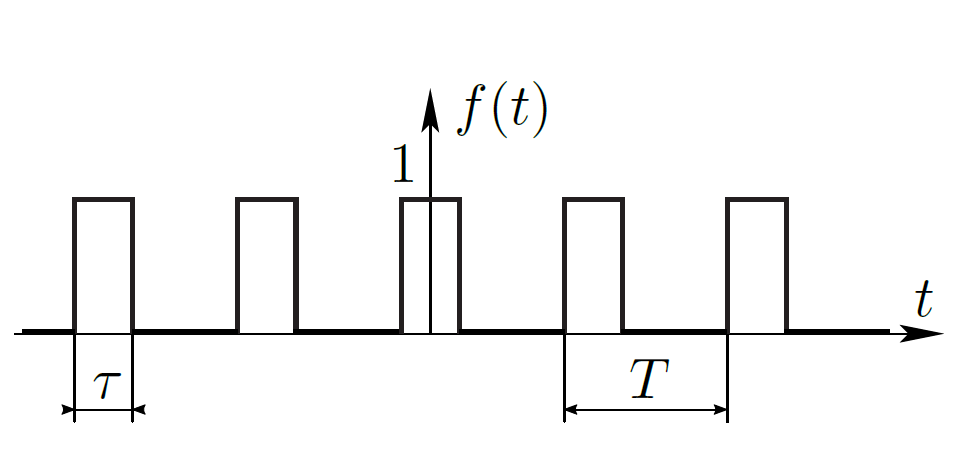
\includegraphics[width=0.4\textwidth]{rect}
\caption{Периодическая последовательность прямоугольных импульсов} \label{rect}
\end{figure}
Рассмотрим спектр периодической последовательности прямоугольных импульсов (рис. \ref{rect}):
\begin{equation}
c_n = \frac{1}{T}\int_{-\tau / 2}^{\tau / 2} e^{-in\omega_0 t}dt = \dfrac{sin(\pi n \tau / T))}{\pi n}
\end{equation}

\subsection*{Свойства спектров}
Справедливо для произвольного сигнала соотношение неопределенностей:
\begin{equation}
\Delta \omega \cdot \Delta t \sim 2\pi
\end{equation}
Рассмотрим спектр обрывка синусоиды (цуг):
\begin{equation}
f(t) = f_0(t)\cos(\omega_0 t)
\end{equation}
Из спектра прямоугольного импульса:
\begin{equation}
F(\omega) = \dfrac{\tau}{2}\left[\dfrac{\sin(\omega-\omega_0)\tau /2}
{(\omega-\omega_0)\tau /2}
 + \dfrac{\sin(\omega+\omega_0)\tau /2}{\omega+\omega_0)\tau /2}\right]
\end{equation}
Получим спектр периодической последовательности цугов (рис. \ref{цуги}):
\begin{equation}
F(\omega) = \dfrac{\tau}{2T}\left[\dfrac{\sin(\omega-\omega_0)\tau /2}
{(\omega-\omega_0)\tau /2}
 + \dfrac{\sin(\omega+\omega_0)\tau /2}{(\omega+\omega_0)\tau /2}\right]
\end{equation}

\begin{figure}[h!]
\begin{center}
\includegraphics[width=0.4\textwidth]{цуги}
\caption{Периодическая последовательность цуг} \label{цуги}
\end{center}
\end{figure}
\subsection*{Модуляция}
Модулированные колебания:
\begin{equation}
f(t) = a(t) \cos (\omega_0 t+\varphi(t))
\end{equation}
Простейшее амплитудно-модулированное колебание:
\begin{equation}
f(t)= a(t) \cos (\omega_0 t), \hspace{3mm} a(t) = a_0(1+m\cos(\Omega t))
\end{equation}
В выражении $0 < m \leq 1$ - глубина модуляции, выражается:
\begin{equation}
m = \dfrac{a_{max}-a_{min}}{a_{max}+a_{min}}
\end{equation}
Из прошлой формулы можно получить:
\begin{equation}
f(t) = a_0 \cos (\omega_0 t) +\dfrac{ma_0}{2}\cos (\omega_0 +\Omega)t++\dfrac{ma_0}{2}\cos (\omega_0 -\Omega)t
\end{equation}

\section{Методика измерений}
В работе используются генератор сигналов произвольной формы, цифровой осциллограф с функцией быстрого преобразования Фурье.

\section{Измерения и обработка данных}
\subsection*{Исследования спектра периодической последовательности прямоугольных импульсов}
На генераторе создается сигнал с разными параметрами, по которому на экране осциллографа получается спектр (рис. \ref{прямоуг})

\begin{figure}[h!]
\begin{minipage}[h!]{0.47\linewidth}
\center{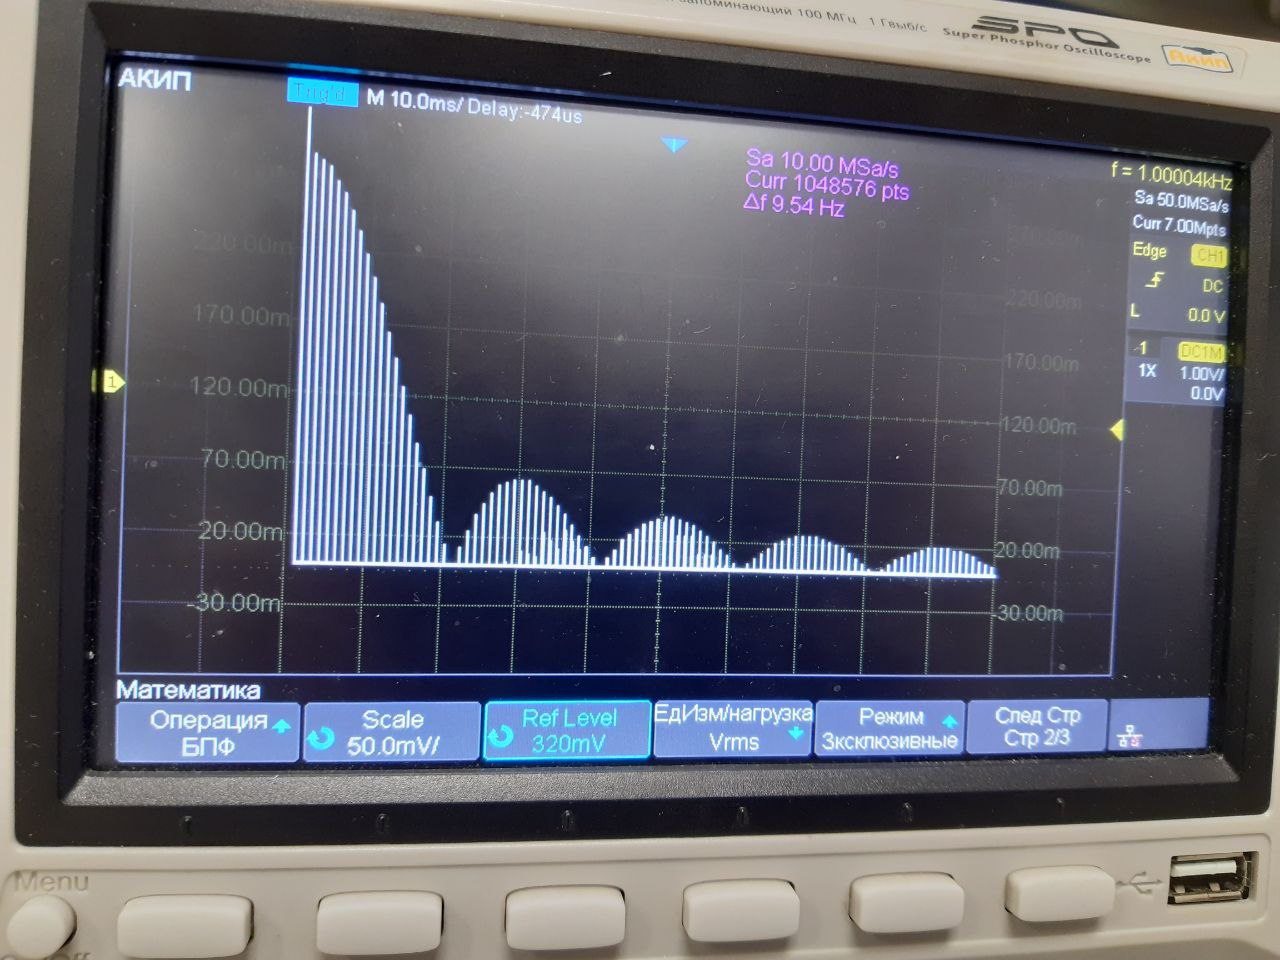
\includegraphics[width=1\linewidth]{1_1}} a) $\nu_{повт} = 1000 Гц, \tau = 50 мкс$\\
\end{minipage}
\hfill
\begin{minipage}[h!]{0.47\linewidth}
\center{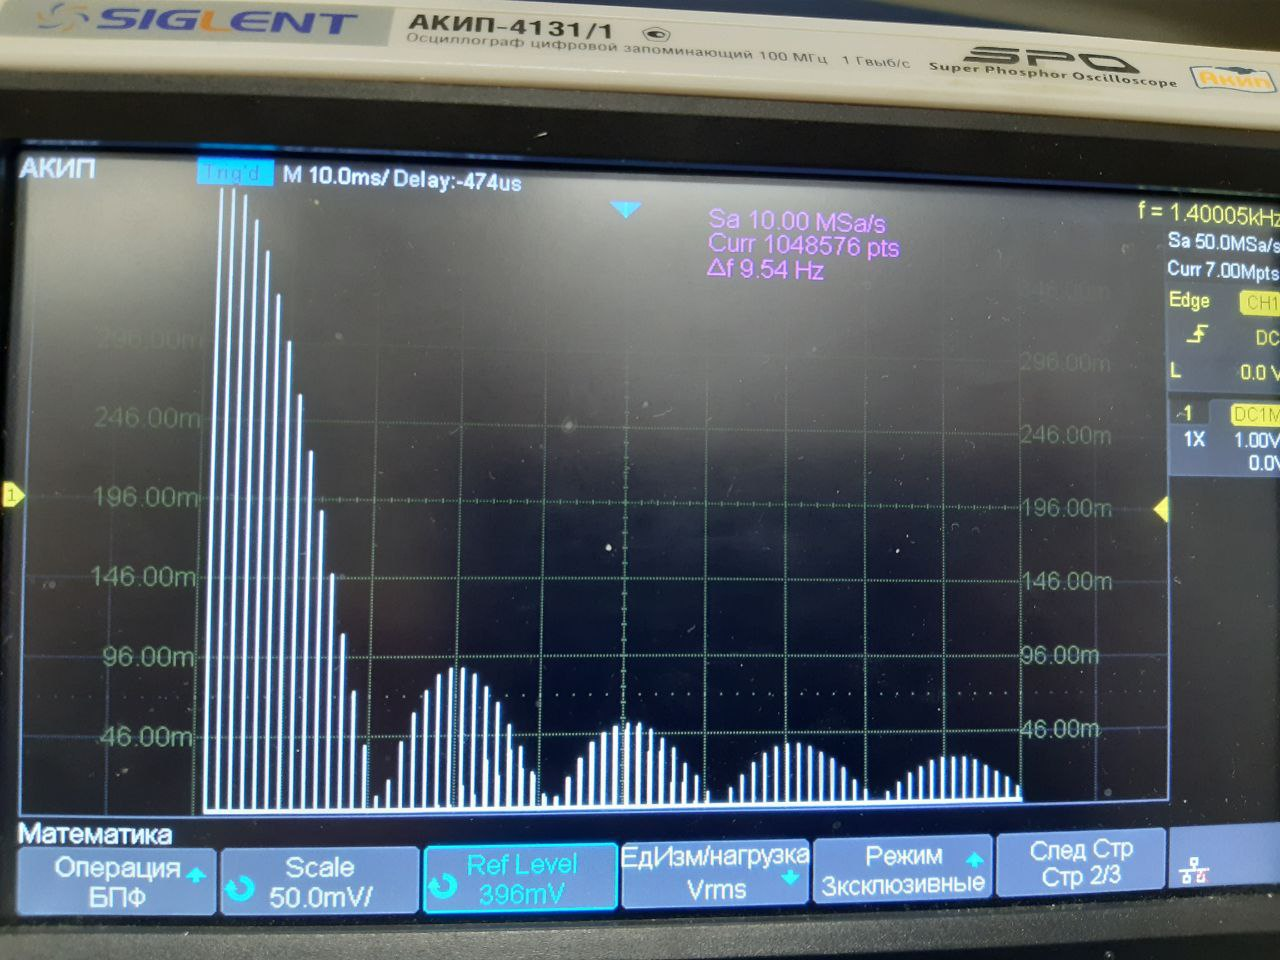
\includegraphics[width=1\linewidth]{1_2}} \\b) $\nu_{повт} = 1400 Гц, \tau = 50 мкс$
\end{minipage}
\vfill
\begin{minipage}[h!]{0.47\linewidth}
\center{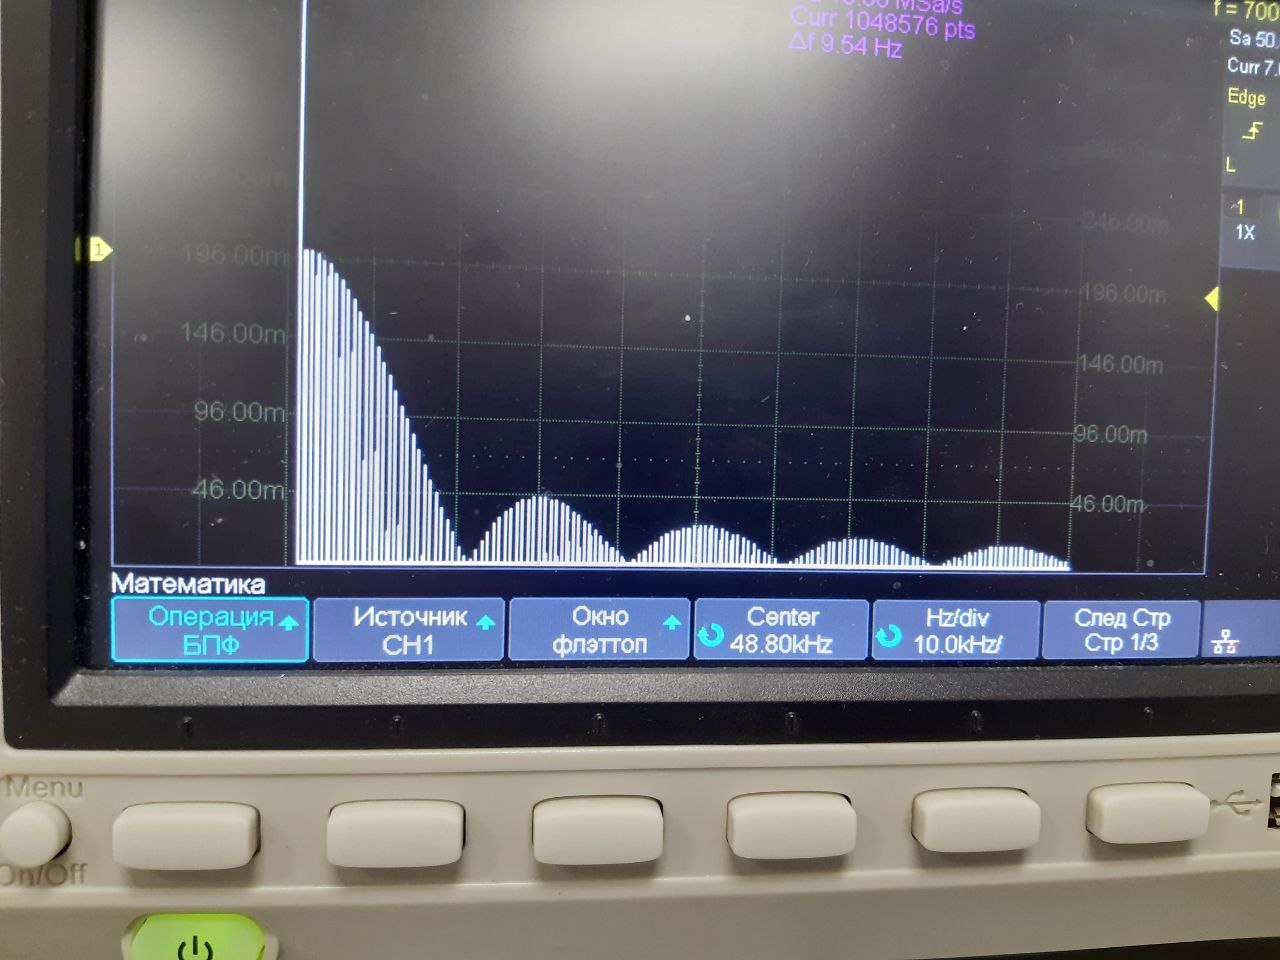
\includegraphics[width=1\linewidth]{1_3}} c) $\nu_{повт} = 700 Гц, \tau = 50 мкс$ \\
\end{minipage}
\hfill
\begin{minipage}[h!]{0.47\linewidth}
\center{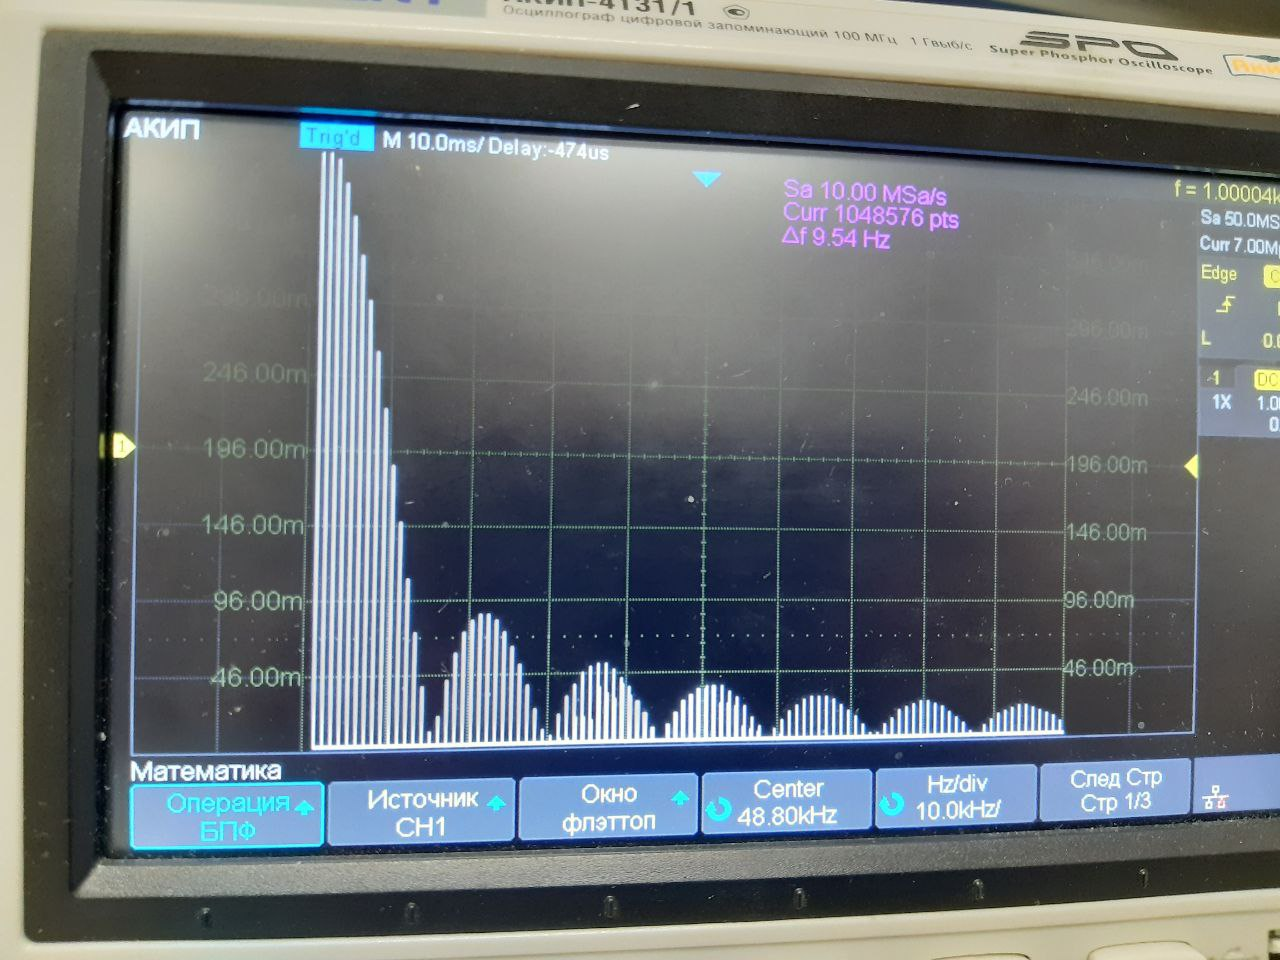
\includegraphics[width=1\linewidth]{1_4}} d) $\nu_{повт} = 1000 Гц, \tau = 70 мкс$ \\
\end{minipage}
\caption{Спектры прямоугольных импульсов}
\label{прямоуг}
\end{figure}
При $\nu_{повт} = 700 Гц$ проведены измерения ширины спектра. Результаты 
представлены в таблице \ref{dnu(tau)_tbl} и на рисунке \ref{dnu(tau)_img}.
\begin{table}[h!]
\caption{Зависимость ширины спектра от длительности спектра} \label{dnu(tau)_tbl}
\begin{tabular}{|l|l|}
\hline
$\Delta\nu$, Hz & $\tau$, мкс \\ \hline
50200         & 20       \\ \hline
25200         & 40       \\ \hline
17200         & 60       \\ \hline
13000         & 80       \\ \hline
10200         & 100      \\ \hline
8600          & 120      \\ \hline
7400          & 140      \\ \hline
6600          & 160      \\ \hline
5800          & 180      \\ \hline
5000          & 200      \\ \hline
\end{tabular}
\end{table}

\begin{figure}[h!]
\begin{center}
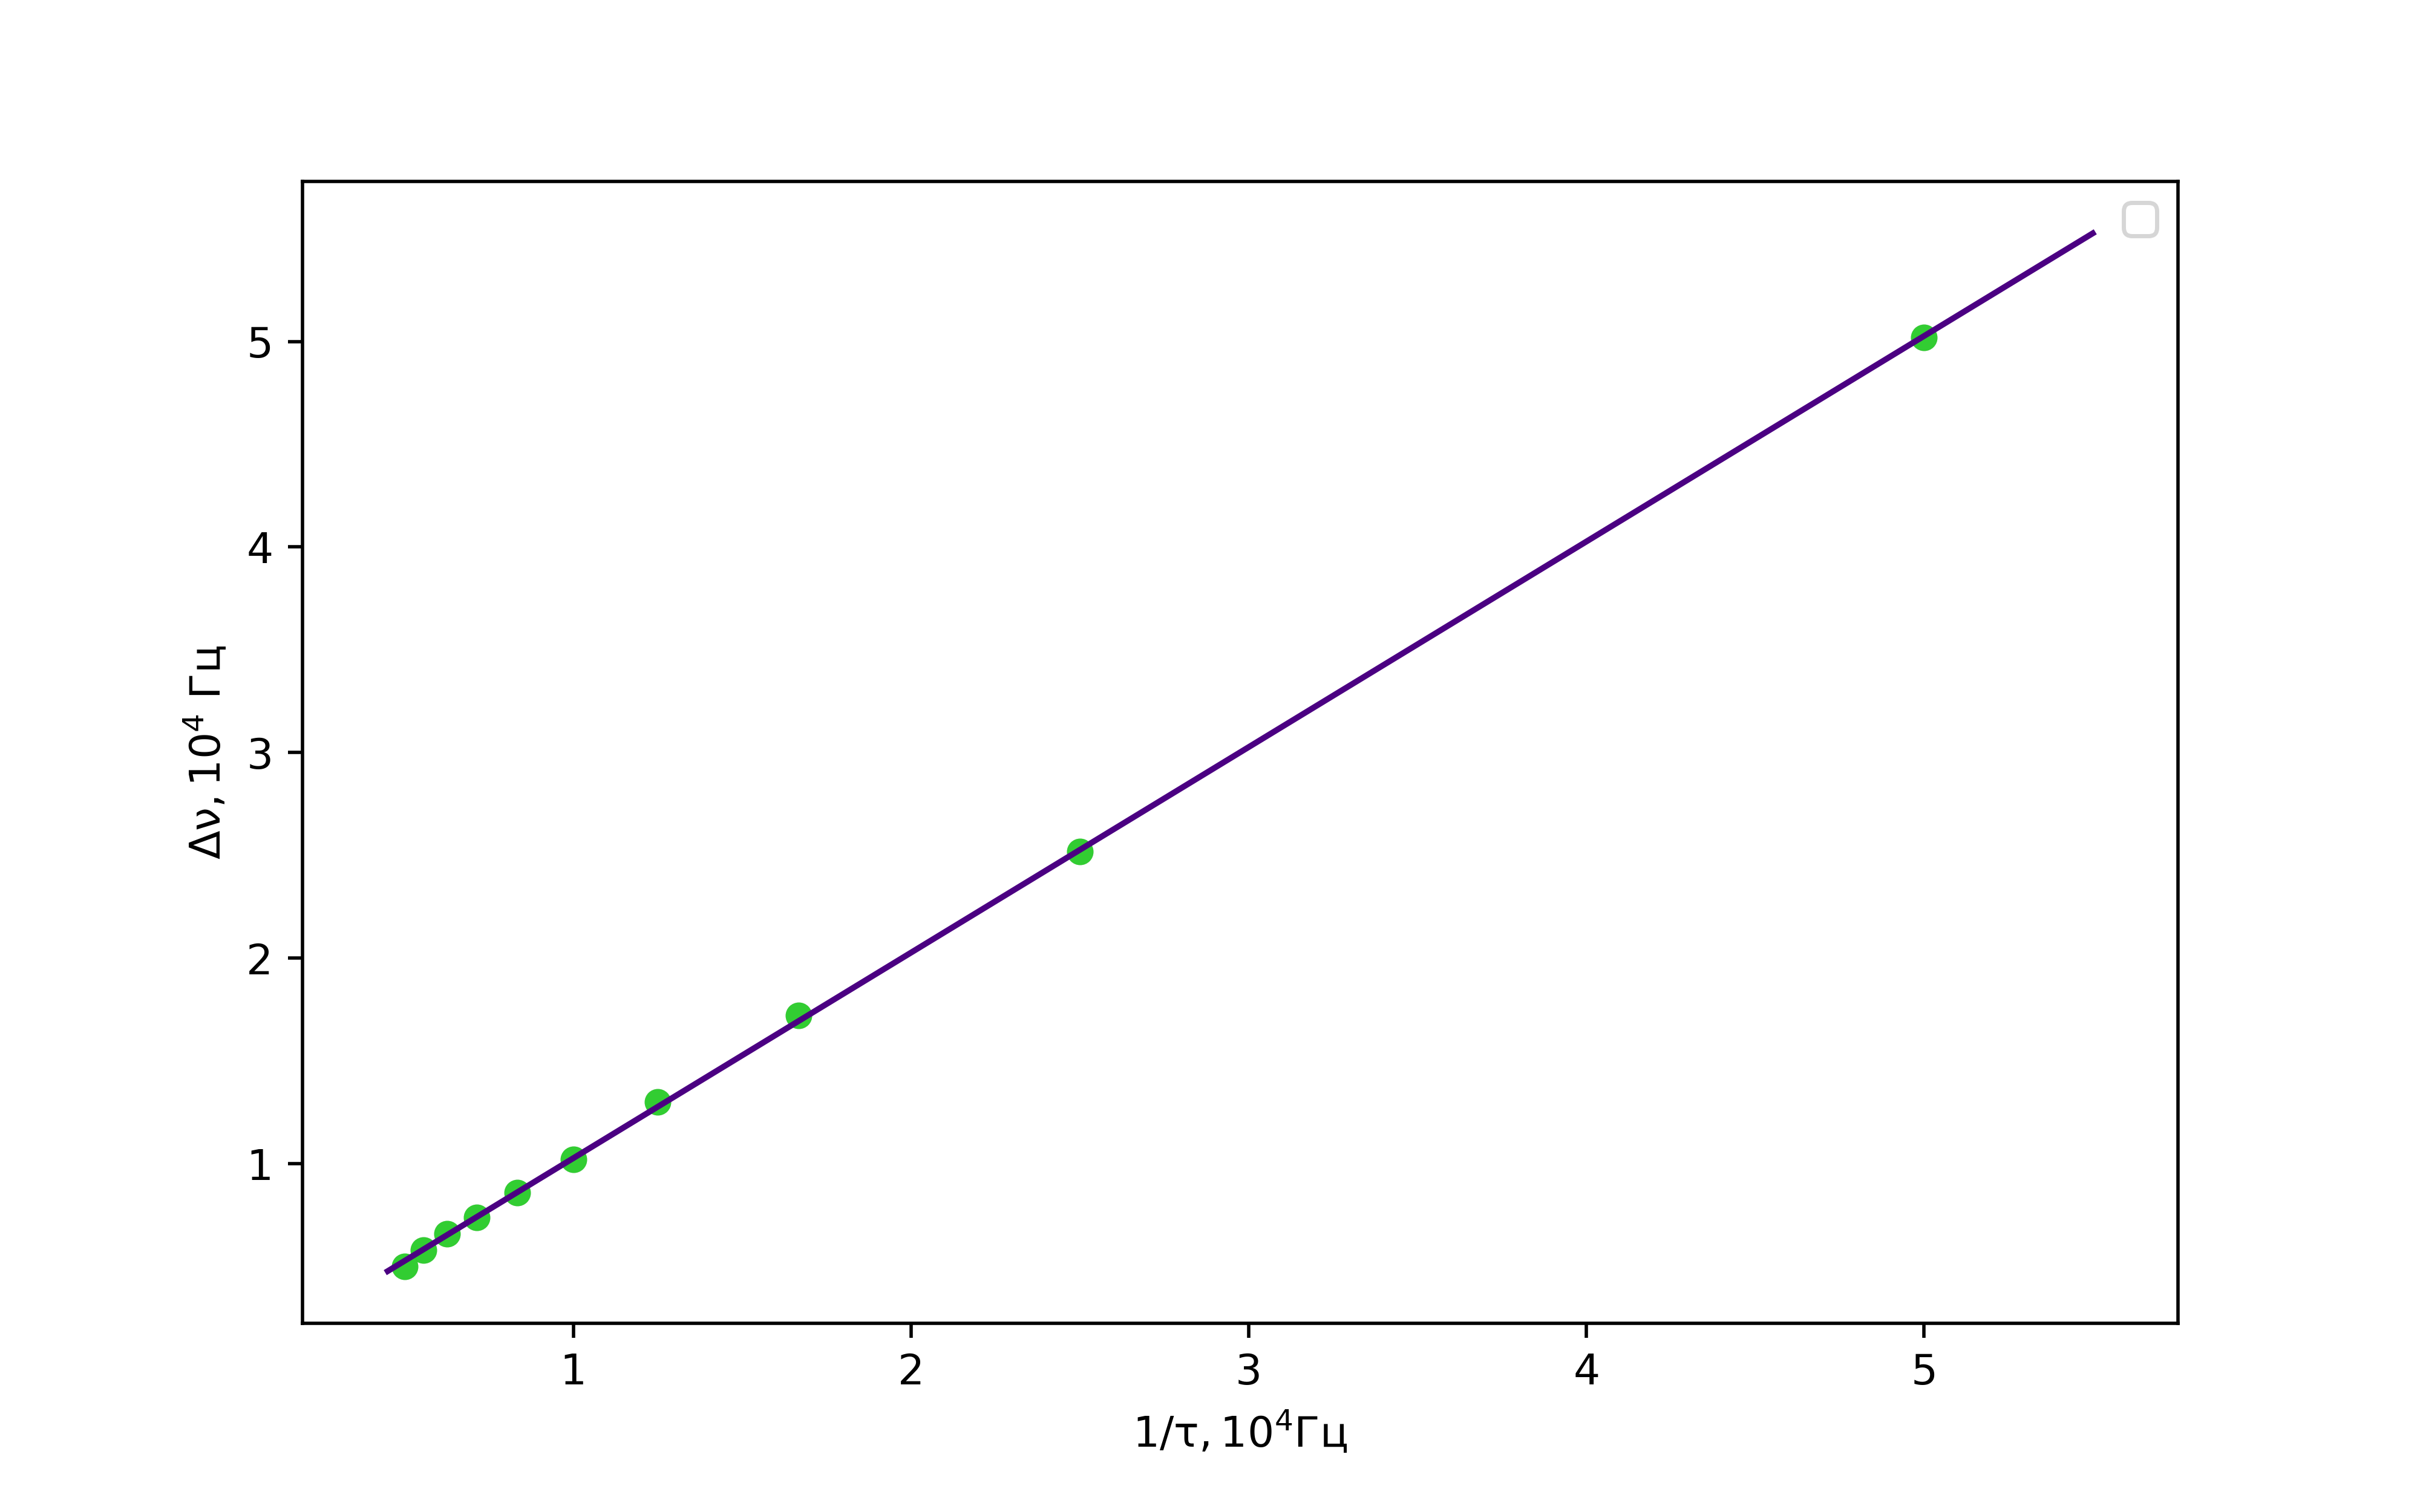
\includegraphics[width=\textwidth]{dnu(tau)}
\caption{Зависимость ширины спектра от длительности спектра} \label{dnu(tau)_img}
\end{center}
\end{figure}
Рассчитаем коэффициент наклона прямой:
\begin{equation}
k = 0.9997 \pm 0.0039
\end{equation}
Полученное значение близко к $1$, что подтверждает соотношение неопределенностей. 


Для одного из сигналов (a) рассчитаем теоретическую зависимость и изобразим на графике \ref{теор}. Теоретический и экспериментальный спектр похожи.

\begin{figure}[h!]
\begin{center}
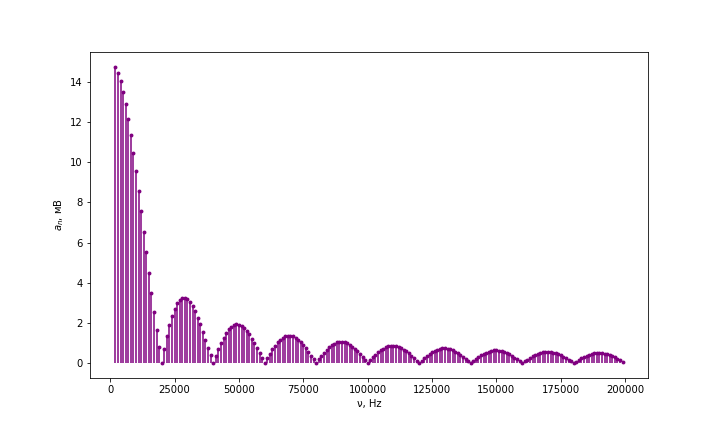
\includegraphics[width=\textwidth]{a(n)}
\caption{Теоретический спектр прямоугольных импульсов} \label{теор}
\end{center}
\end{figure}

\subsection{Исследование спектра периодической последовательности цугов гармонических колебаний}
На генераторе создается сигнал последовательности синусоидальных цугов с разными параметрами, по которому на экране осциллографа получается спектр. (рис. \ref{спектр_цуги})

\begin{figure}[h!]
\begin{minipage}[h!]{0.47\linewidth}
\center{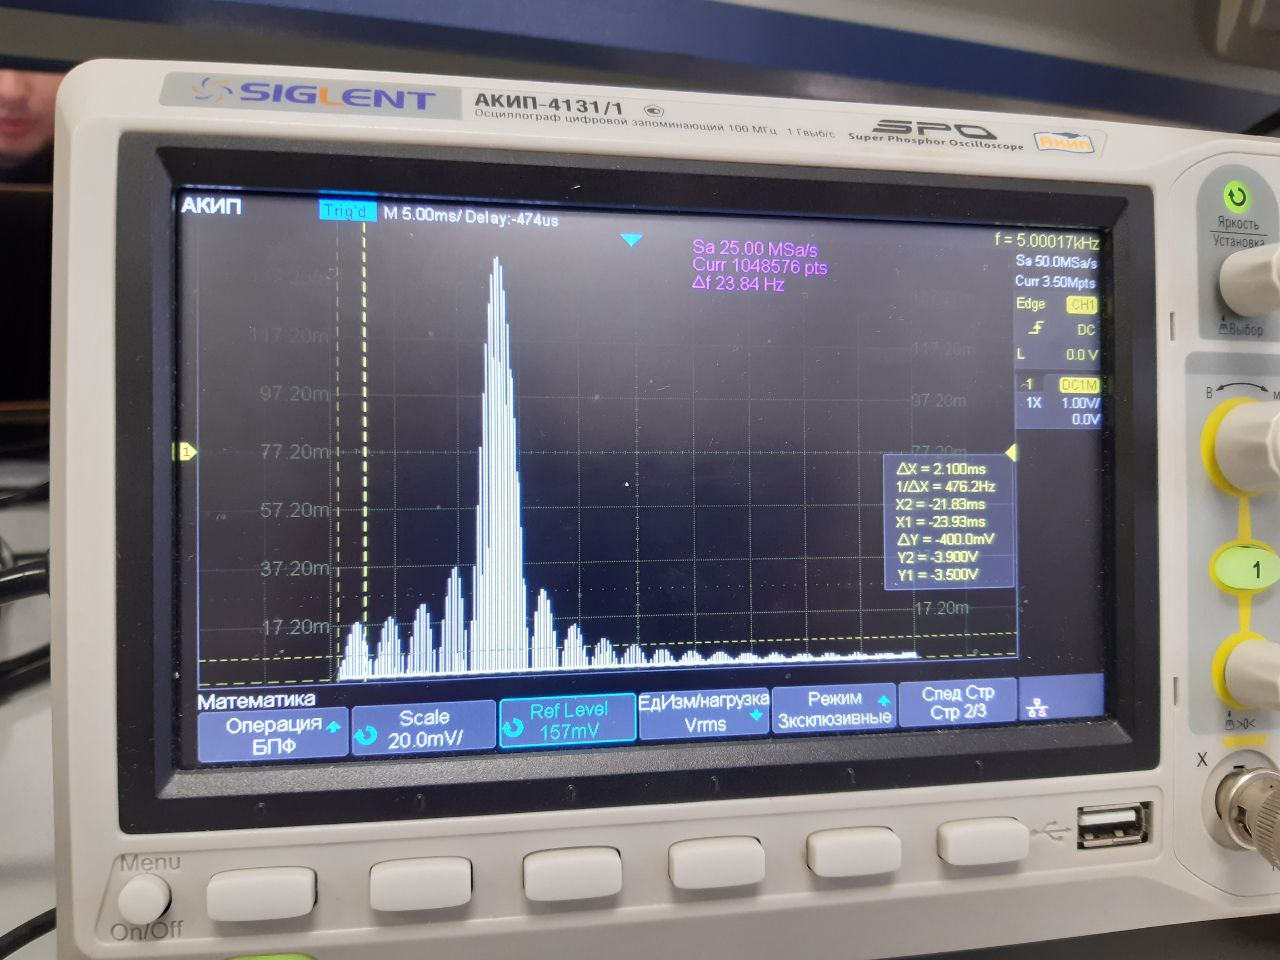
\includegraphics[width=1\linewidth]{2_1}} a) $\nu = 50 кГц, T = 1 мс, N = 5$\\
\end{minipage}
\hfill
\begin{minipage}[h!]{0.47\linewidth}
\center{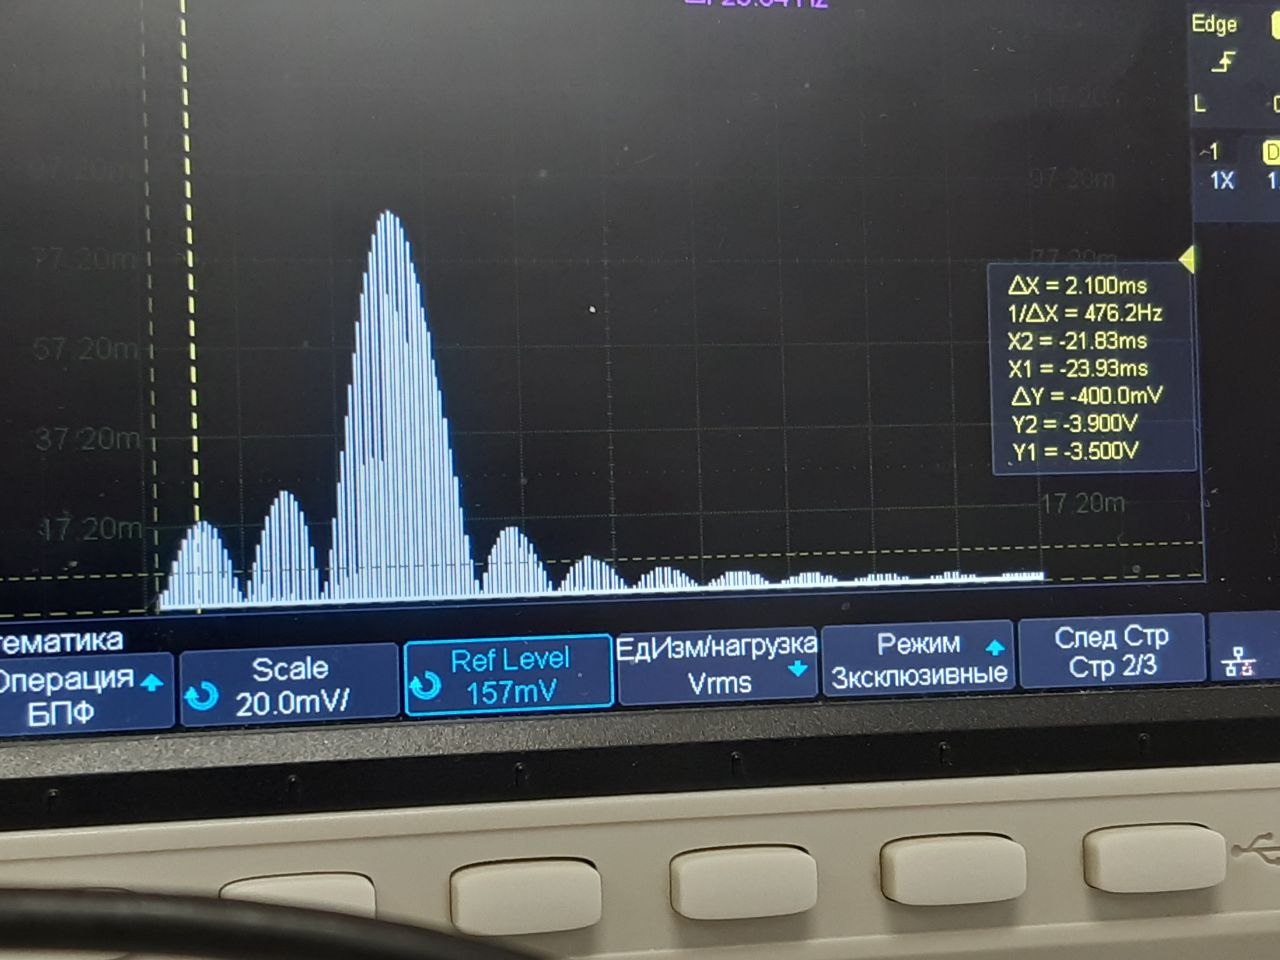
\includegraphics[width=1\linewidth]{2_2}} \\b) $\nu = 50 кГц, T = 1 мс, N = 3$
\end{minipage}
\vfill
\begin{minipage}[h!]{0.47\linewidth}
\center{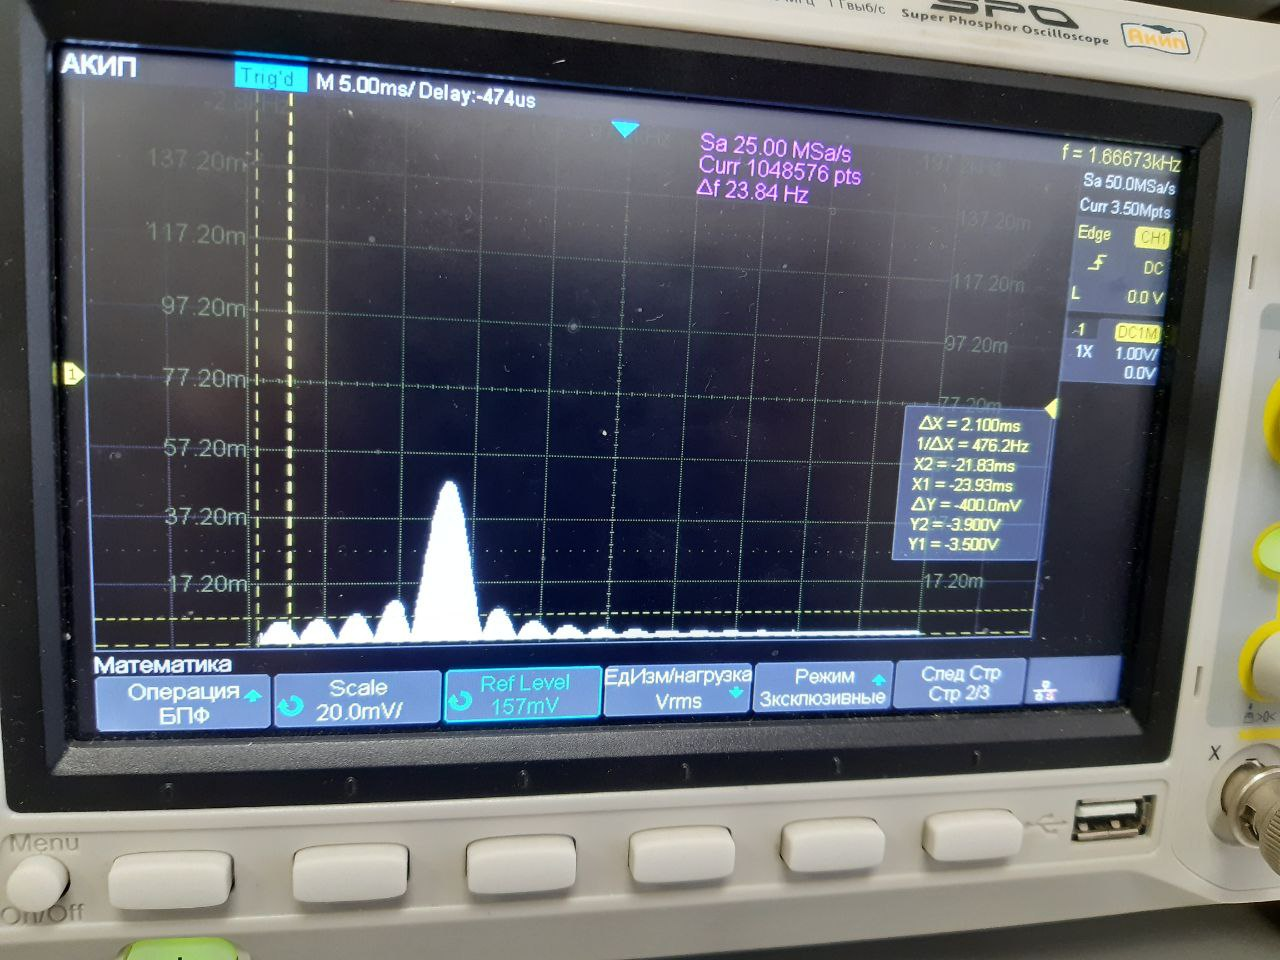
\includegraphics[width=1\linewidth]{2_3}} c) $\nu = 50 кГц, T = 3 мс, N = 5$ \\
\end{minipage}
\hfill
\begin{minipage}[h!]{0.47\linewidth}
\center{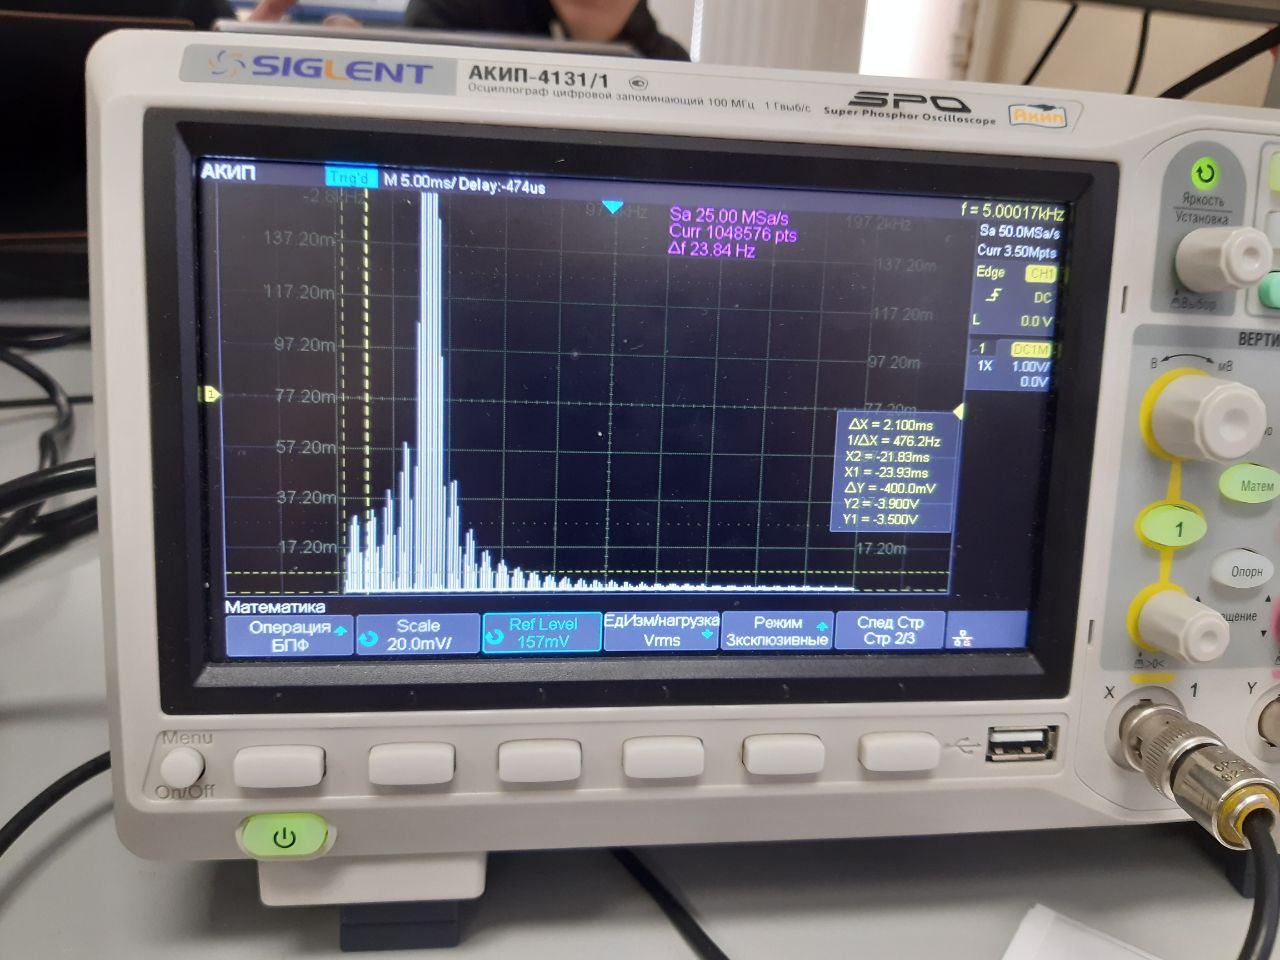
\includegraphics[width=1\linewidth]{2_4}} d) $\nu = 30 кГц, T = 1 мс, N = 5$ \\
\end{minipage}
\vfill
\begin{minipage}[h!]{0.47\linewidth}
\center{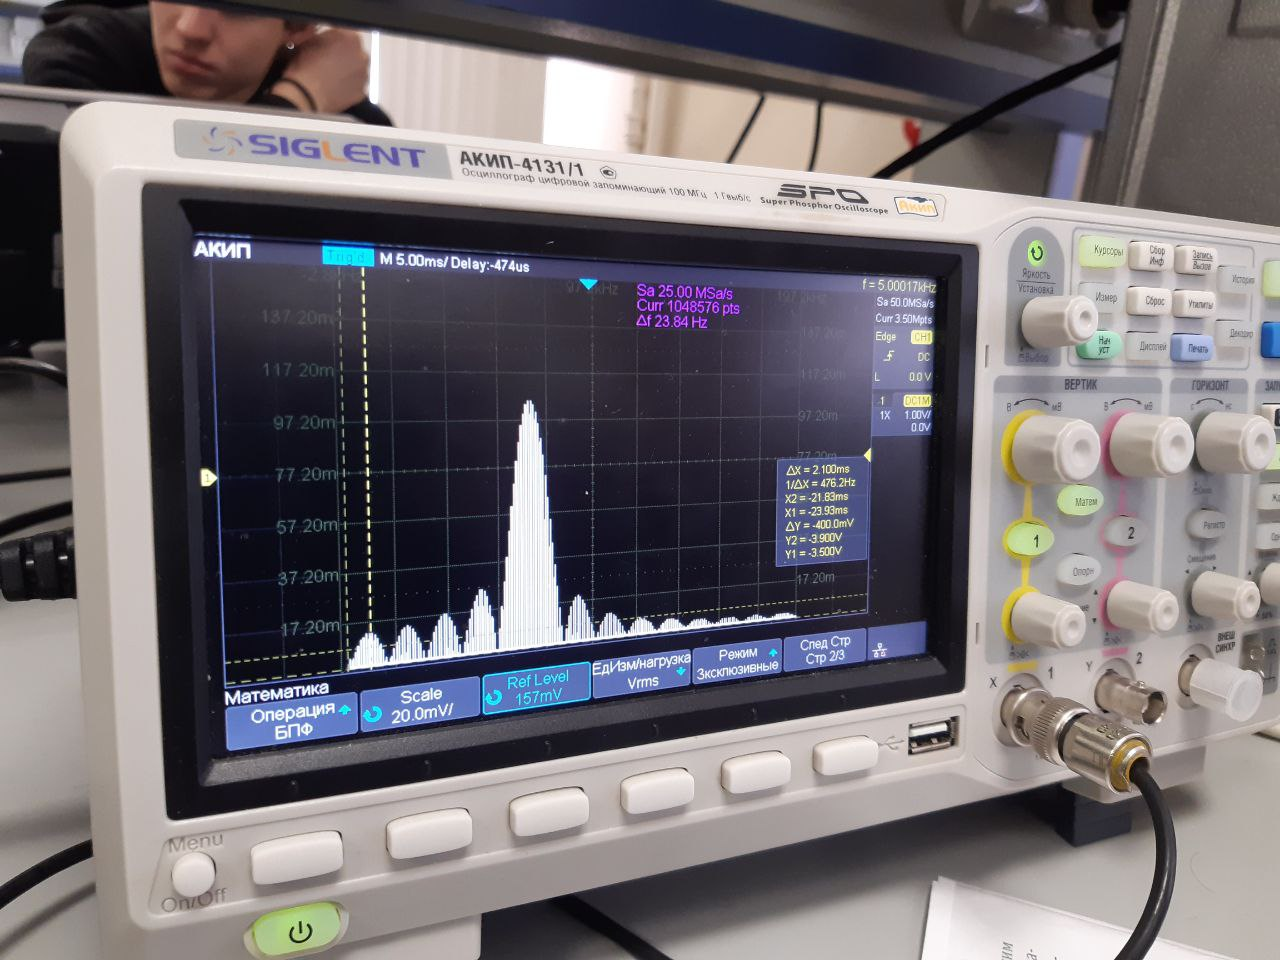
\includegraphics[width=1\linewidth]{2_5}} \\e) $\nu = 70 кГц, T = 1 мс, N = 5$
\end{minipage}
\caption{Вид спектра при разных параметрах спектра}
\label{спектр_цуги}
\end{figure}

При фиксированной длительности импульсов $\tau$ = 50 мкс измерим расстояния между соседними спектральными компонентами от периода повторения импульсов (табл. \ref{dnu(T)_tbl}, рис. \ref{dnu(T)_img})

\begin{table}[h!]
\caption{Зависимость расстояния между соседними спектральными компонентами от периода повторения импульсов} \label{dnu(T)_tbl}
\begin{tabular}{|l|l|}
\hline
T, ms & $\delta \nu$, Hz \\ \hline
0.2   & 6250    \\ \hline
1     & 2778    \\ \hline
1.5   & 4167    \\ \hline
2     & 1042    \\ \hline
2.5   & 1190    \\ \hline
3     & 735     \\ \hline
3.5   & 893     \\ \hline
4     & 1000    \\ \hline
4.5   & 1042    \\ \hline
5     & 1190    \\ \hline
\end{tabular}
\end{table}

\begin{figure}[h!]
\begin{center}
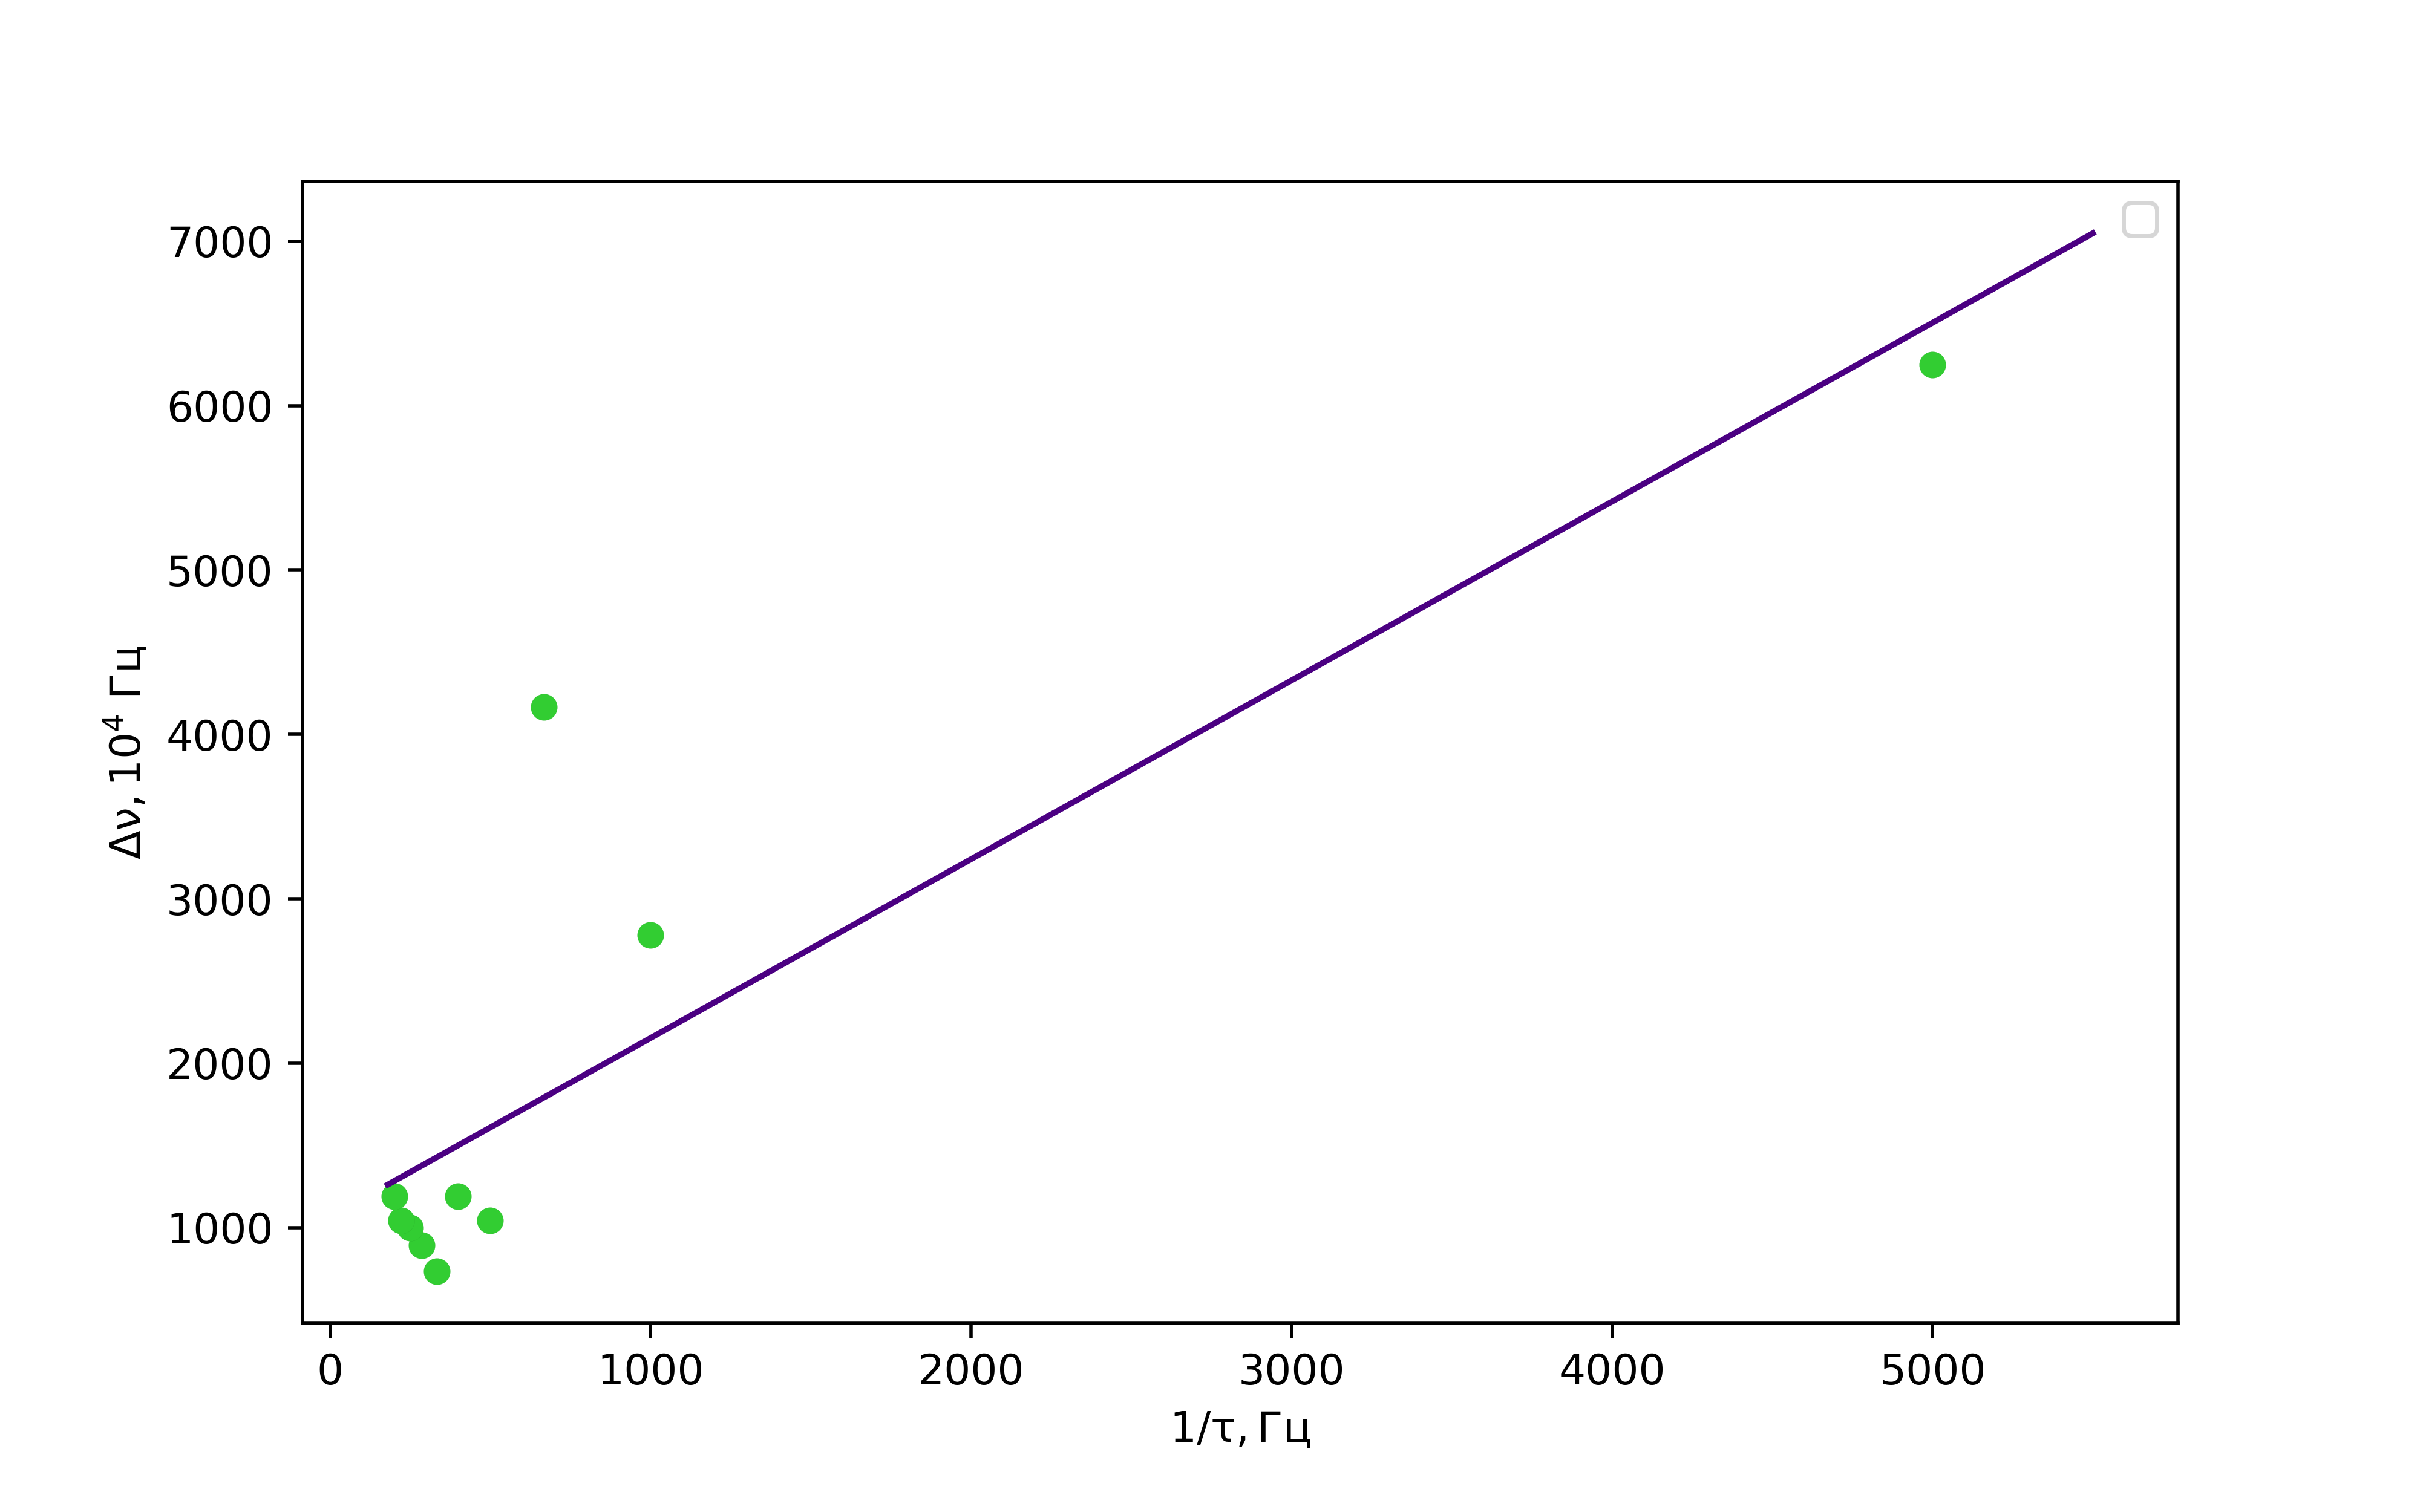
\includegraphics[width=0.9\textwidth]{T(dnu)}
\caption{Зависимость расстояния между соседними спектральными компонентами от периода повторения импульсов} \label{dnu(T)_img}
\end{center}
\end{figure}

Точки должны хорошо ложиться на прямую, однако из графика видно, что это не так. Проблема заключается в снятии данных (был выбран неверный канал при курсорных измерениях). Поэтому подтвердить справедливость соотношения неопределенности невозможно. 

\subsection{Исследование спектра гармонических сигналов, модулированных по амплитуде}
На генераторе создается сигнал, модулированных по амплитуде, по которому на экране осциллографа получается спектр (\ref{мод}).
\begin{figure}[h!]
\begin{center}
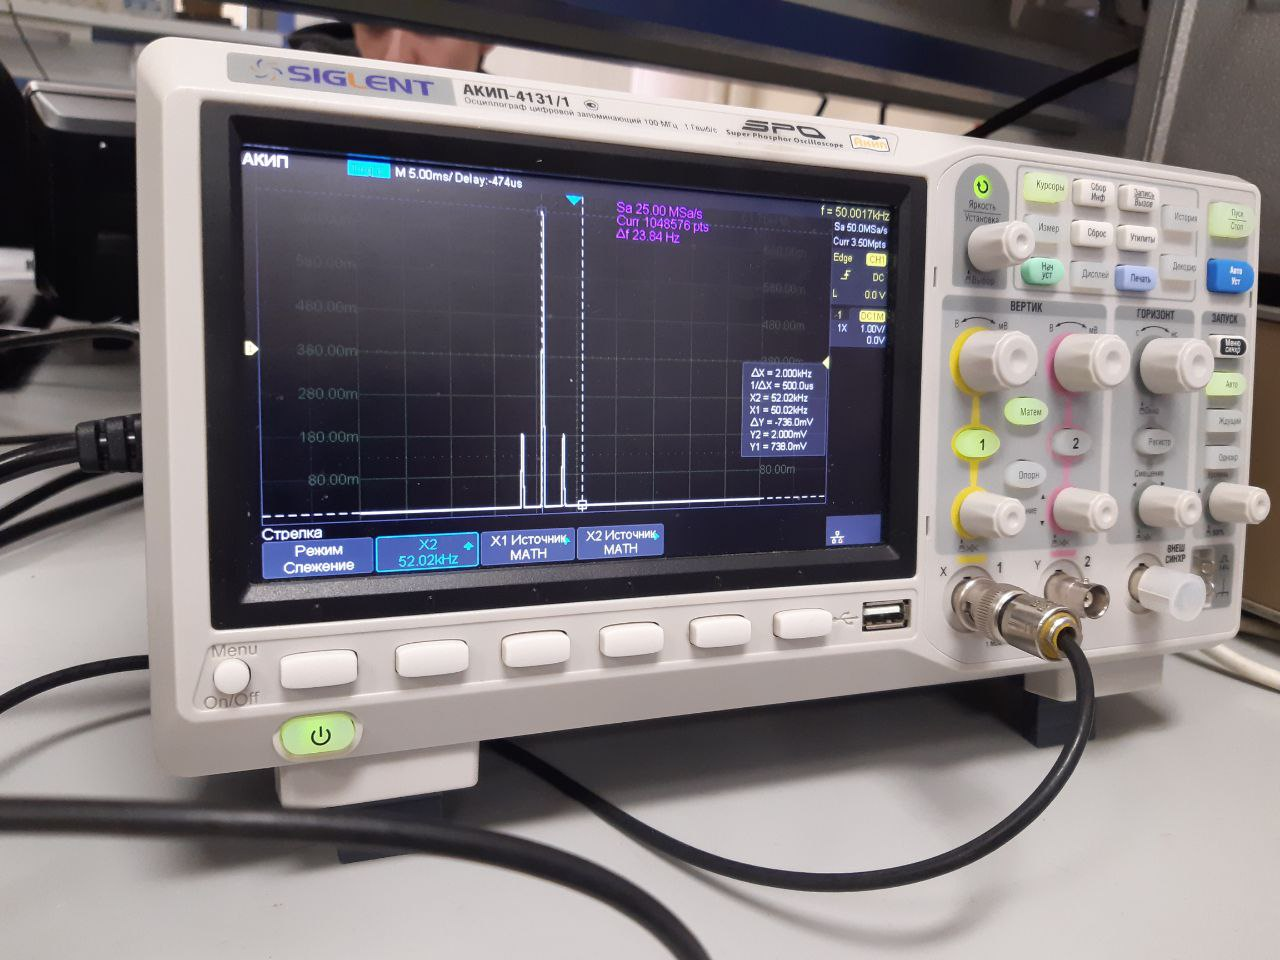
\includegraphics[width=\textwidth]{3}
\caption{Спектр сигнала, модулированного по амплитуде} \label{мод}
\end{center}
\end{figure}
Измерим с помощью осциллографа глубину модуляции:
\begin{equation}
m = \dfrac{A_{max}-A_{min}}{A_{max}+A_{min}} = \dfrac{1.54 - 0.04}{1.54 + 0.04} = 0.5, что сходится с установленным на генераторе
\end{equation}
Изменяя глубину модуляции, измерим $\dfrac{a_{бок}}{а_{осн}}$ (табл. \ref{mod_tbl} и рис. \ref{mod_img}).

\begin{table}[h!]
\caption{Зависимость $\dfrac{a_{бок}}{а_{осн}}$ от $m$}
\label{mod_tbl}
\begin{tabular}{|l|l|l|}
\hline
m   & a\_бок & a\_центр \\ \hline
50  & 186    & 738      \\ \hline
10  & 38     & 738      \\ \hline
20  & 74     & 738      \\ \hline
30  & 110    & 738      \\ \hline
40  & 150    & 738      \\ \hline
60  & 222    & 738      \\ \hline
70  & 258    & 738      \\ \hline
80  & 298    & 738      \\ \hline
90  & 334    & 738      \\ \hline
100 & 370    & 738      \\ \hline
\end{tabular}
\end{table}
\begin{figure}[h!]
\begin{center}
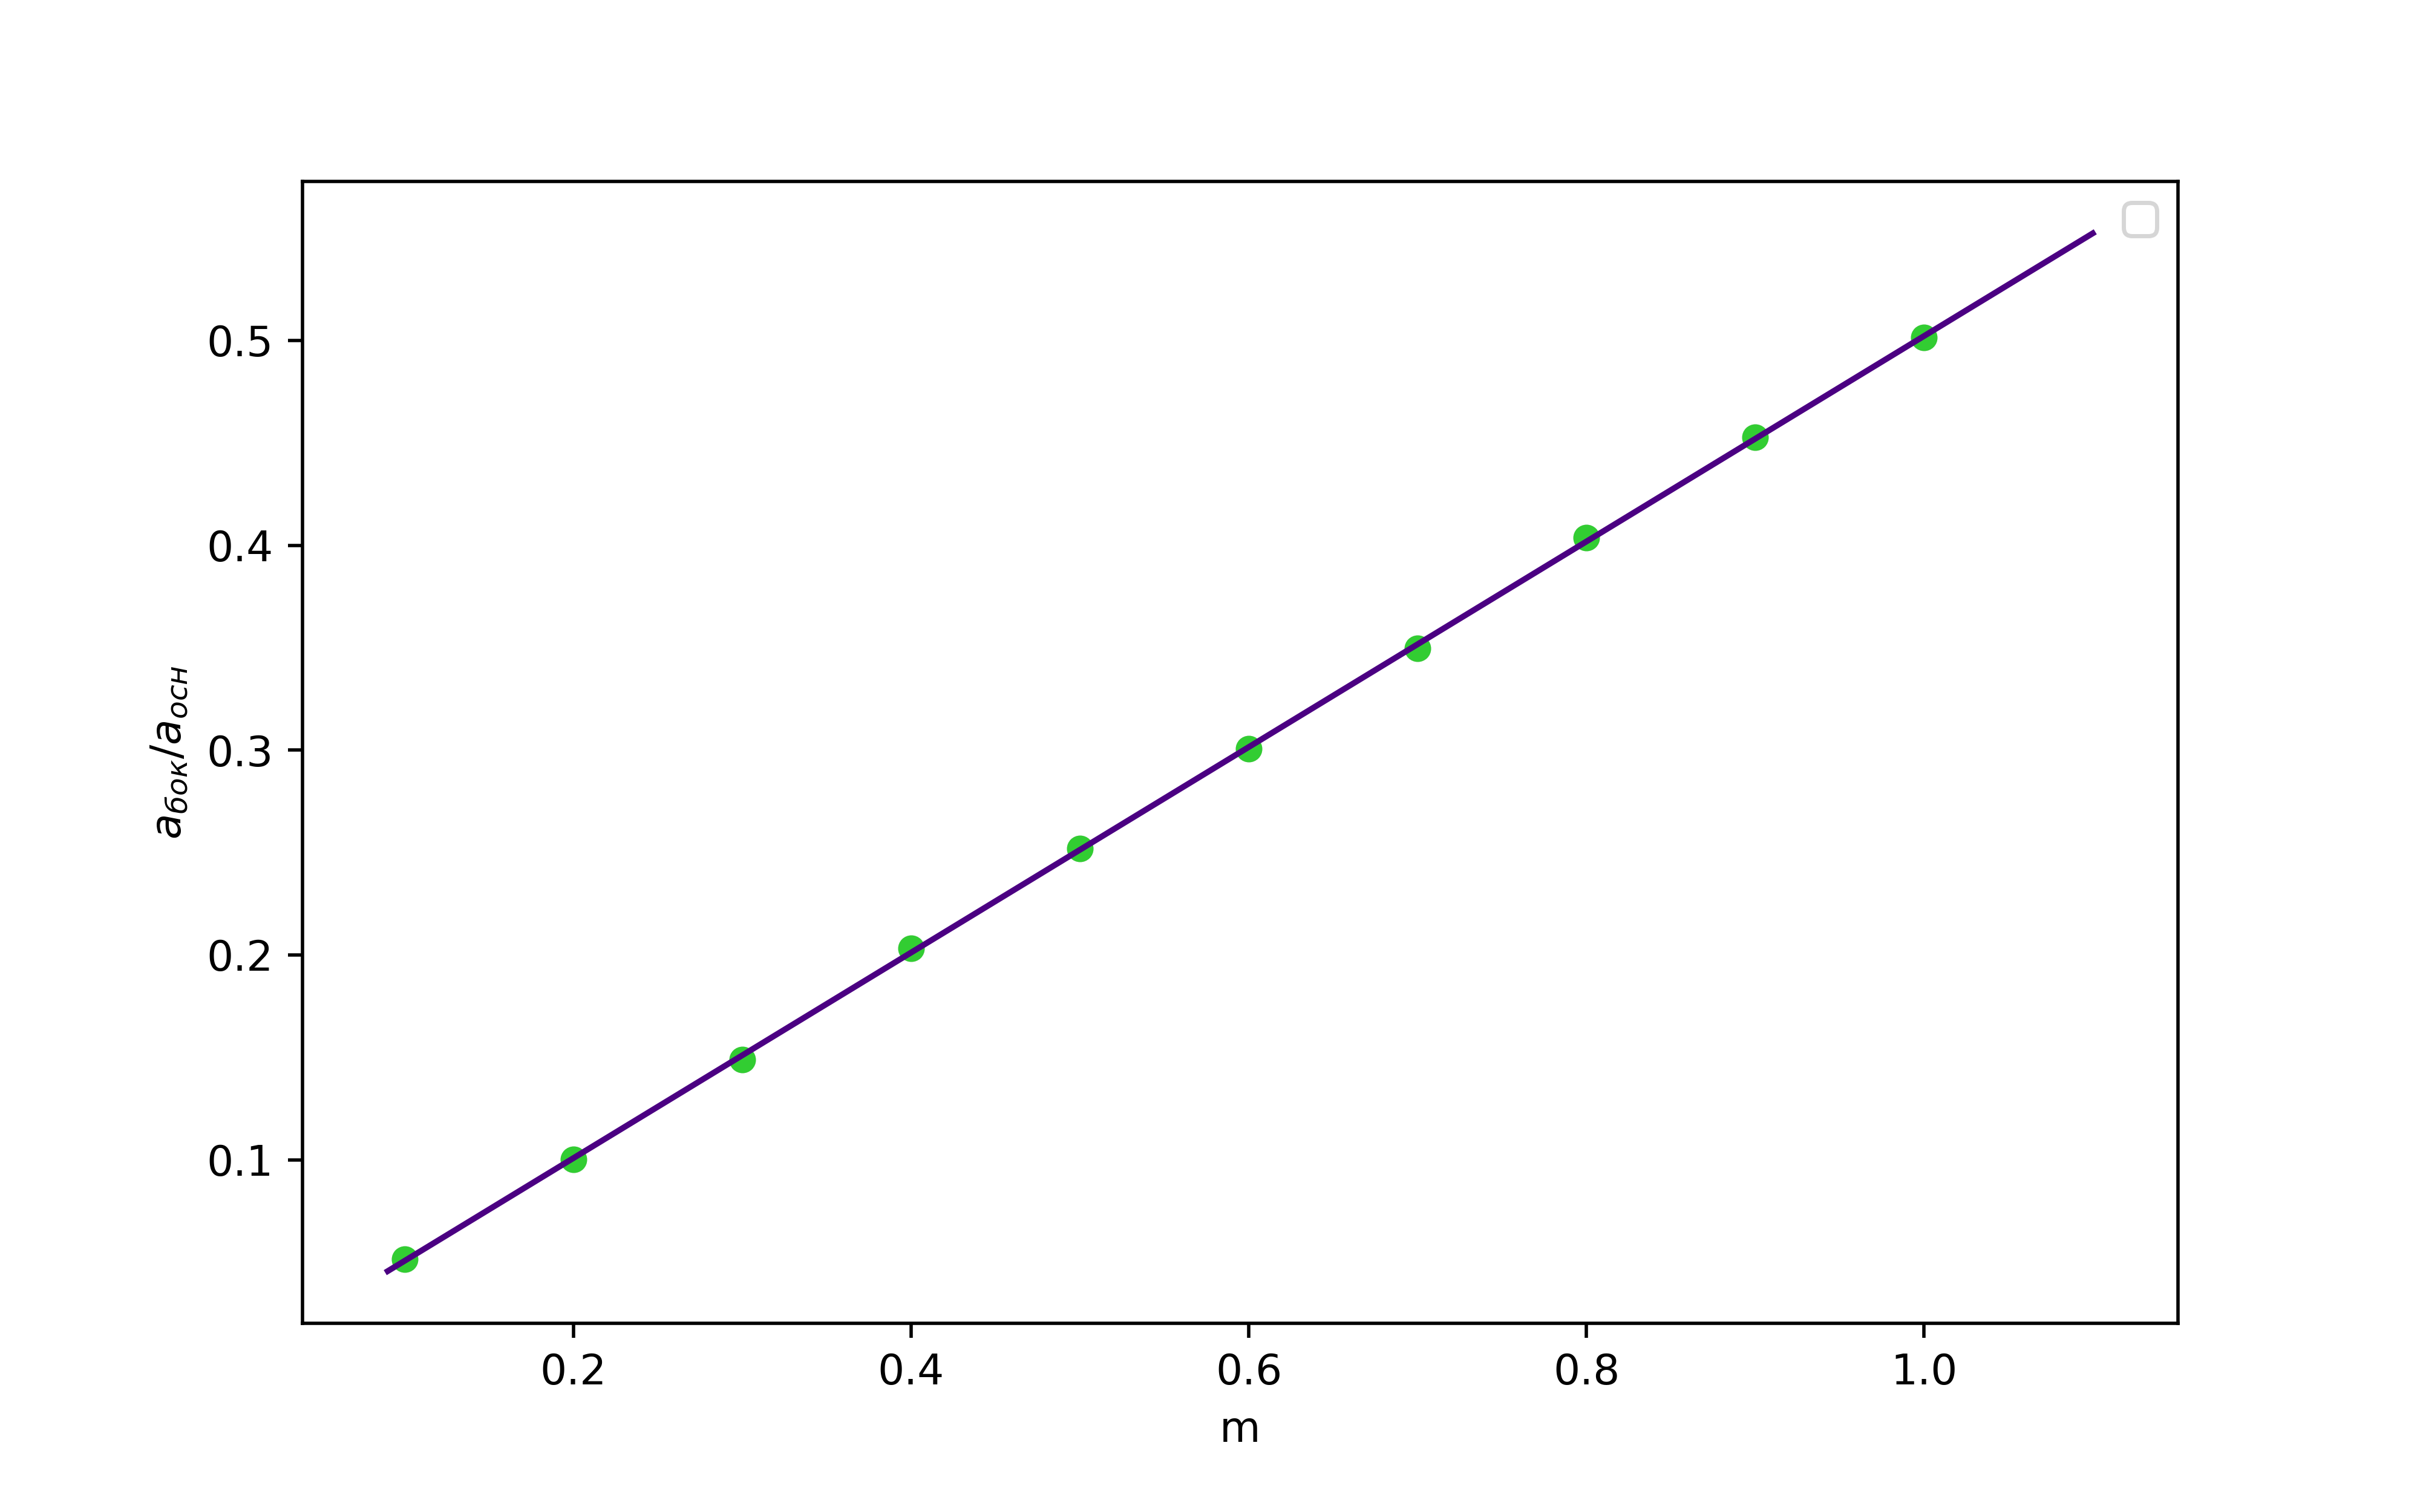
\includegraphics[width=0.9\textwidth]{a(m)}
\caption{Зависимость $\dfrac{a_{бок}}{а_{осн}}$ от $m$} \label{mod_img}
\end{center}
\end{figure}
Определим коэффициент наклона прямой:
\begin{equation}
k = 0.502 \pm 0.002
\end{equation} 
Результат сходится с предсказанным теоретически (0.5).

\section{Выводы}


1. При исследовании последовательности прямоугольных импульсов получена зависимость ширины спектра от длительности импульса, что подтверждает соотношение неопределенностей: $\tau \cdot \Delta\nu \sim 1$.

2. Проверены теоретические расчеты спектра при прямоугольных импульсах (теоретическая и экспериментальная картины схожи).

3. При обработке данных от спектра периодической последовательности цугов была обнаружена ошибка при снятии данных, что не позволило проверить соотношение неопределенностей.

4. Получен угол наклона графика зависимости $\dfrac{a_{бок}}{а_{осн}}$ от $m$ (0.5), подтверждено теоретическое значение этого угла (0.5).

\end{document}